\chapter{Demostración}
En este capítulo se mostrará una pequeña demostración del uso de la aplicación que haría cualquier usuario de la aplicación. Además de establecer un test para comprobar que la lógica de los algoritmos del buscador está correctamente implementada.

\section{Pruebas unitarias}
Para una correcta metodología, es necesario contar con una serie de test unitarios que permitan comprobar cada vez que se añade una nueva funcionalidad, la correcta integración de la misma. En el proyecto actual solo existe una funcionalidad, pero se deja la puerta abierta para el desarrollo de nuevas utilidades en el futuro, como añadir cualquier restricción alimentaria que pueda tener el usuario, cambiando los ingredientes problemáticos por unos permitidos para el usuario. 

Para los test, se añaden los pertinentes que permiten realizar comprobar que lo que ve el usuario es lo correcto en cada momento, no solo comprobando si se devuelve un código de respuesta correcto (2xx) sino que realmente sea lo que el usuario tiene que estar viendo, haciendo los test a nivel de vista.

En el desarrollo de las pruebas se ha realizado con la herramienta pytest, incluida en \Gls{django}. Se ha generado un \gls{test} para cada filtro de la base de datos.
\begin{enumerate}
    \item Recetas
    \begin{itemize}
        \item Identificador
        \item Nombre
        \item Ingredientes
    \end{itemize}
    \item Ingredientes
    \begin{itemize}
        \item Identificador
        \item Nombre
    \end{itemize}
\end{enumerate}

Para ejecutar los \gls{test} se hace uso de la tarea especificada para ello en Invoke, el código de las pruebas se incluye en el anexo de la documentación. 

\begin{figure}
    \centering
    \begin{lstlisting}[style=consola]
        invoke test
    \end{lstlisting}
    \caption{Comando para lanzar los test unitarios}
    \label{sni:test}
\end{figure}

\section{Prueba de la aplicación}
En esta sección se hará una prueba completa a la aplicación, desde el punto de vista del usuario, relatando el viaje por la aplicación de uno de los usuarios: Daniel Pérez.

Daniel encuentra un anuncio de la aplicación en internet y se anima a probarla ya que se le suelen caducar algunos ingredientes de la despensa. Al entrar en la aplicación, desde su ordenador personal, se encuentra directamente con el buscador principal. Echa un vistazo a la \gls{interfaz}, pensando en las recetas aleatorias que aparecen a la derecha. Entrando en una porque parece que tiene buena pinta, lamentablemente no cuenta con los ingredientes para realizarla y vuelve al buscador principal. 

\newpage
\begin{figure}
    \centering
    \fbox{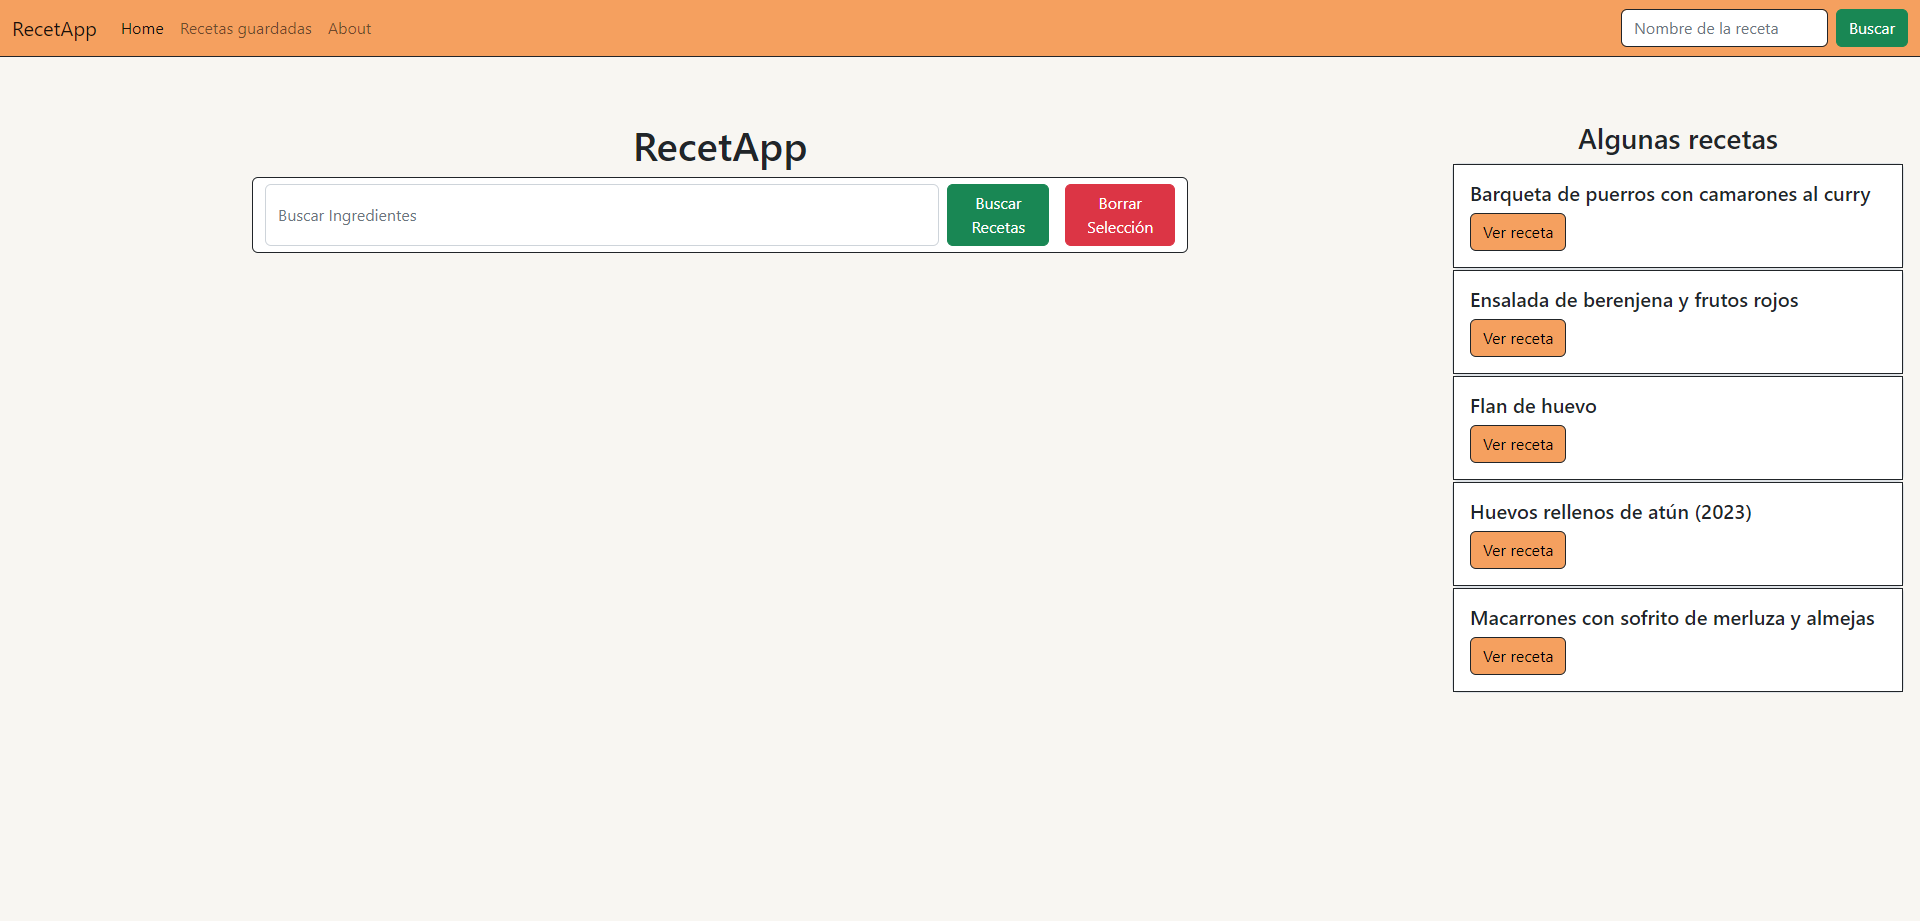
\includegraphics[width=125mm, scale=1]{./doc/imagenes/home_escritorio.png}}
    \fbox{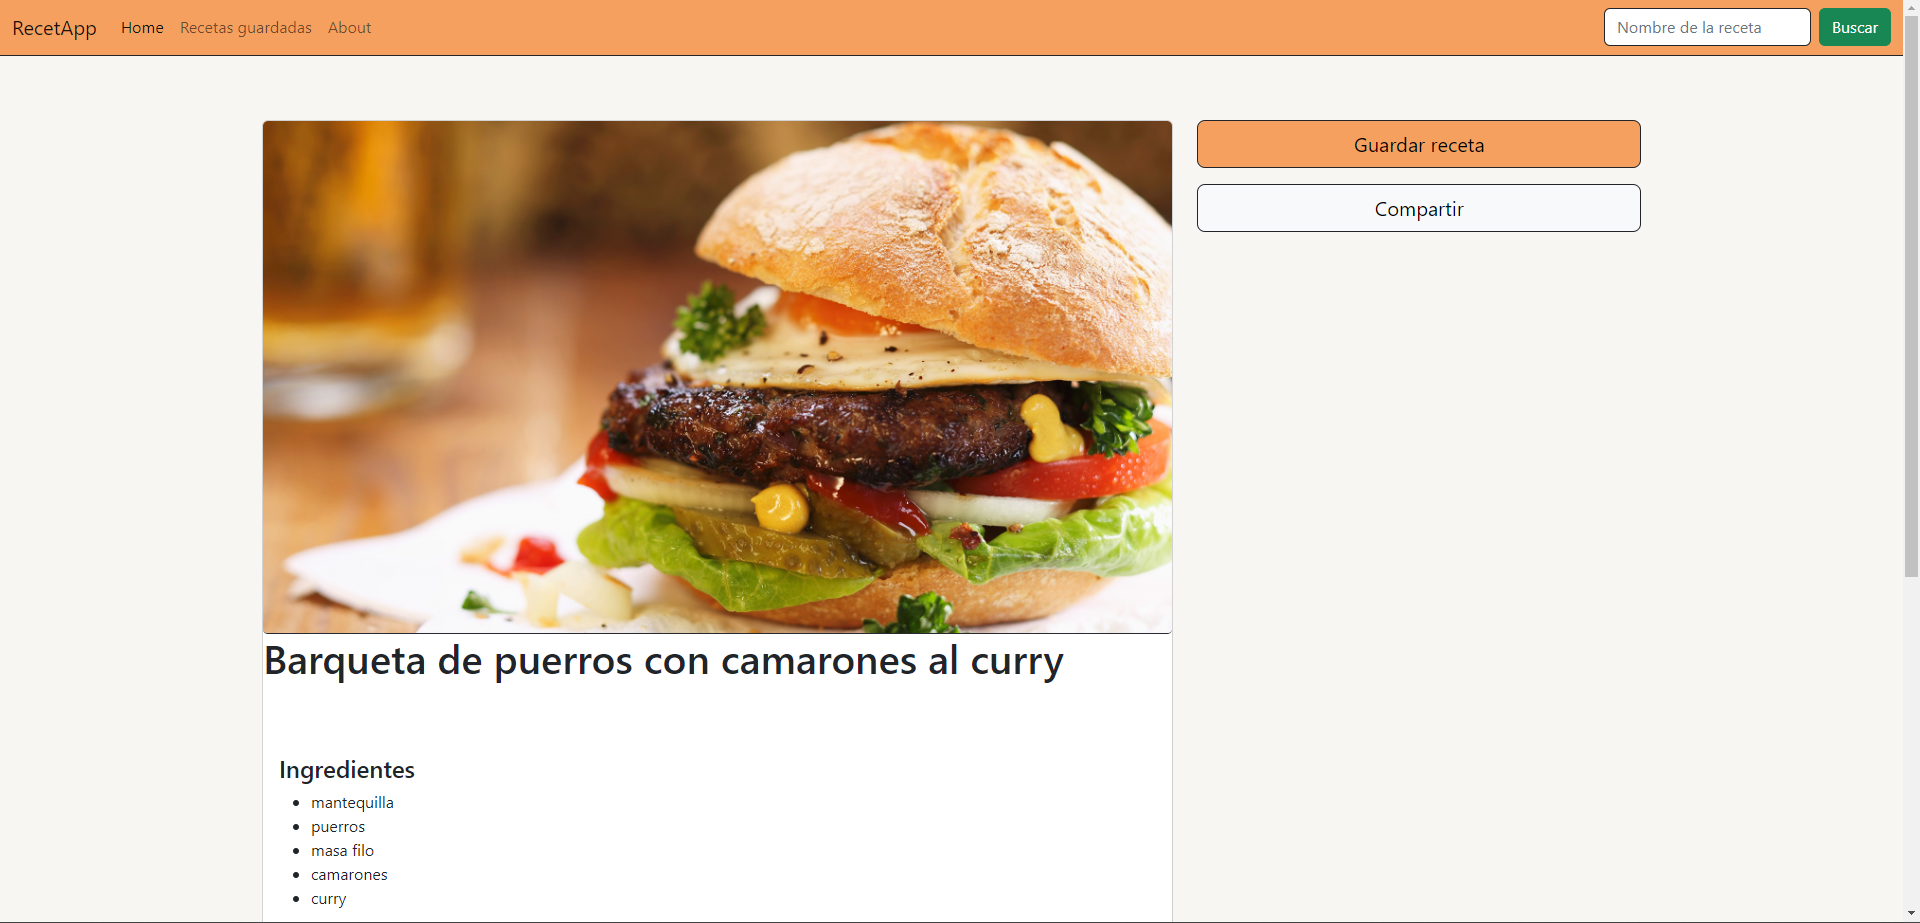
\includegraphics[width=125mm, scale=1]{./doc/imagenes/Receta_Daniel.png}}
    \caption{Primeros pasos de Daniel}
    \label{fig:Daniel-pasos1}
\end{figure}

Una vez que vuelve a la página principal, empieza a introducir los ingredientes que quiere gastar. Como últimamente quiere comer sano, le apetece cenar una pescado, gastando las espinacas que están a punto de caducar y añadiendo otros ingredientes que le sobran.
\begin{enumerate}
    \item Bacalao
    \item Huevos
    \item Espinacas
    \item Nata
    \item Leche evaporada
    \item Limón
    \item Queso en polvo
    \item mantequilla
\end{enumerate}

El buscador debería encontrar las recetas que usan estos ingredientes, mostrándolas al usuario de manera organizada y clara.

Daniel pulsa el botón para buscar ingredientes con el botón verde habilitado para ello. Los resultados que ha obtenido son los esperados, ha obtenido todas las recetas que se esperaba que devolviera la aplicación. 

Daniel mira los resultados devueltos y elige comer un budín de bacalao, seleccionando dicha receta desde el buscador, leyendo la receta y reuniendo los ingredientes para realizar los pasos detallados. 
\begin{figure}[h!]
    \centering
    \fbox{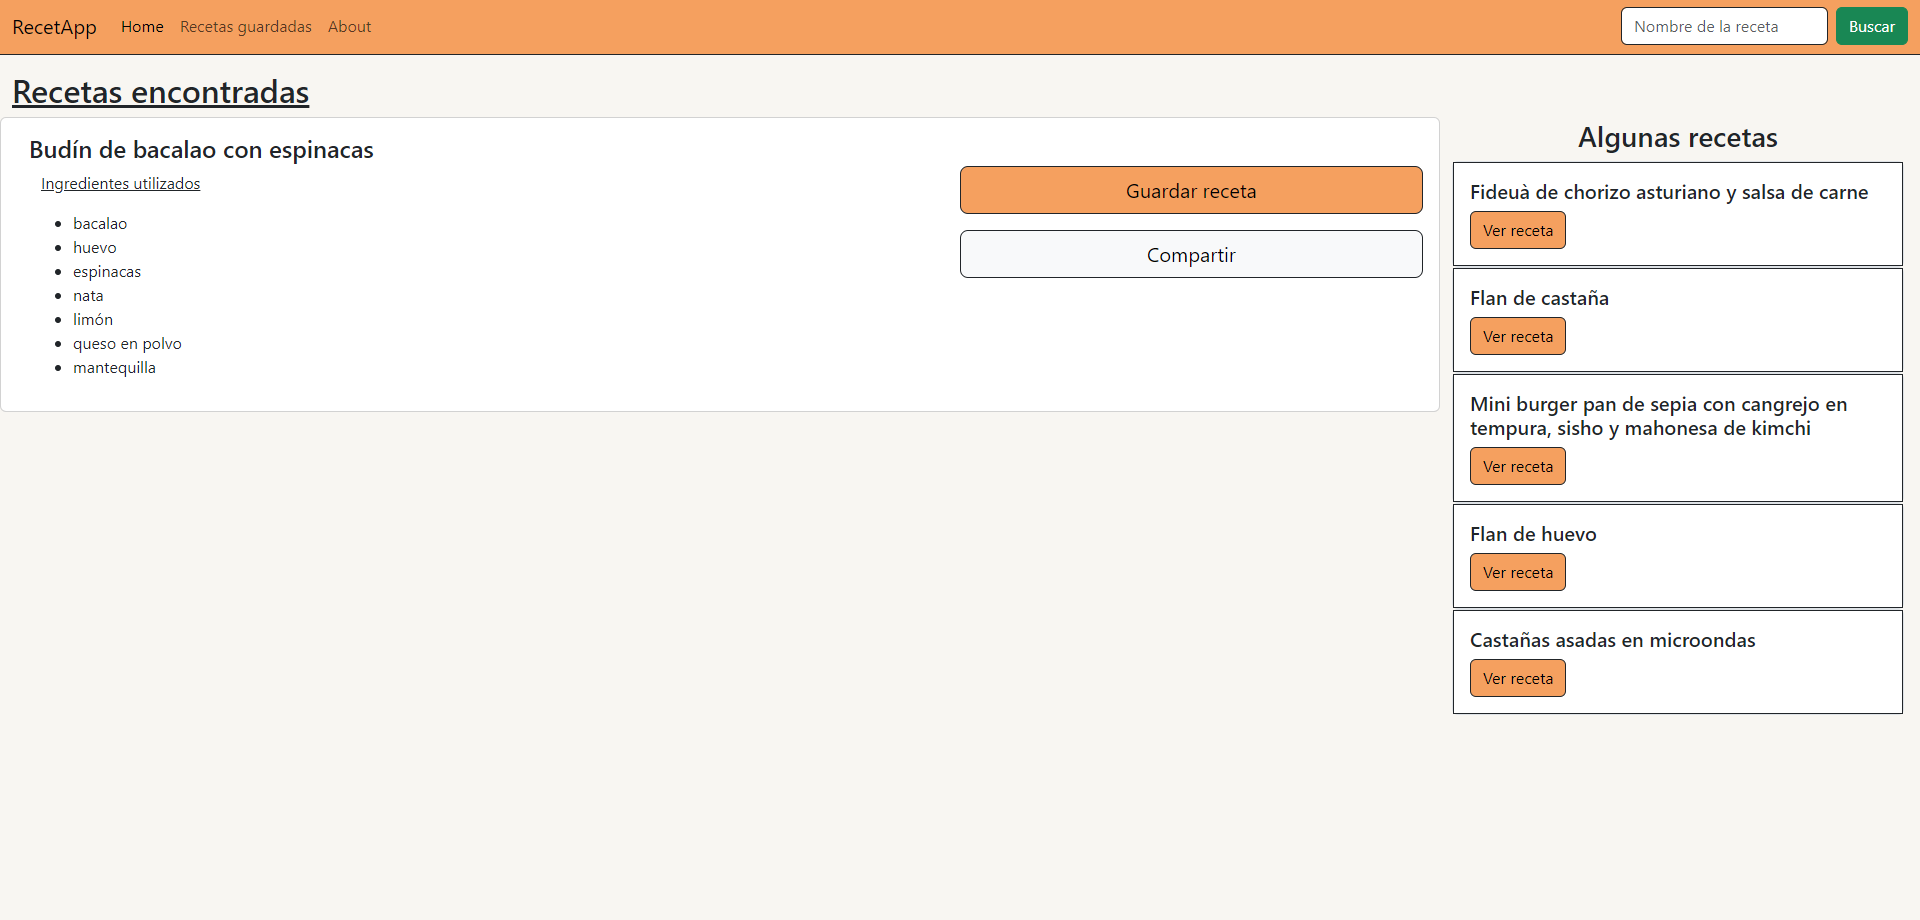
\includegraphics[width=120mm, scale=1]{./doc/imagenes/Resultados_Daniel.png}}
    \fbox{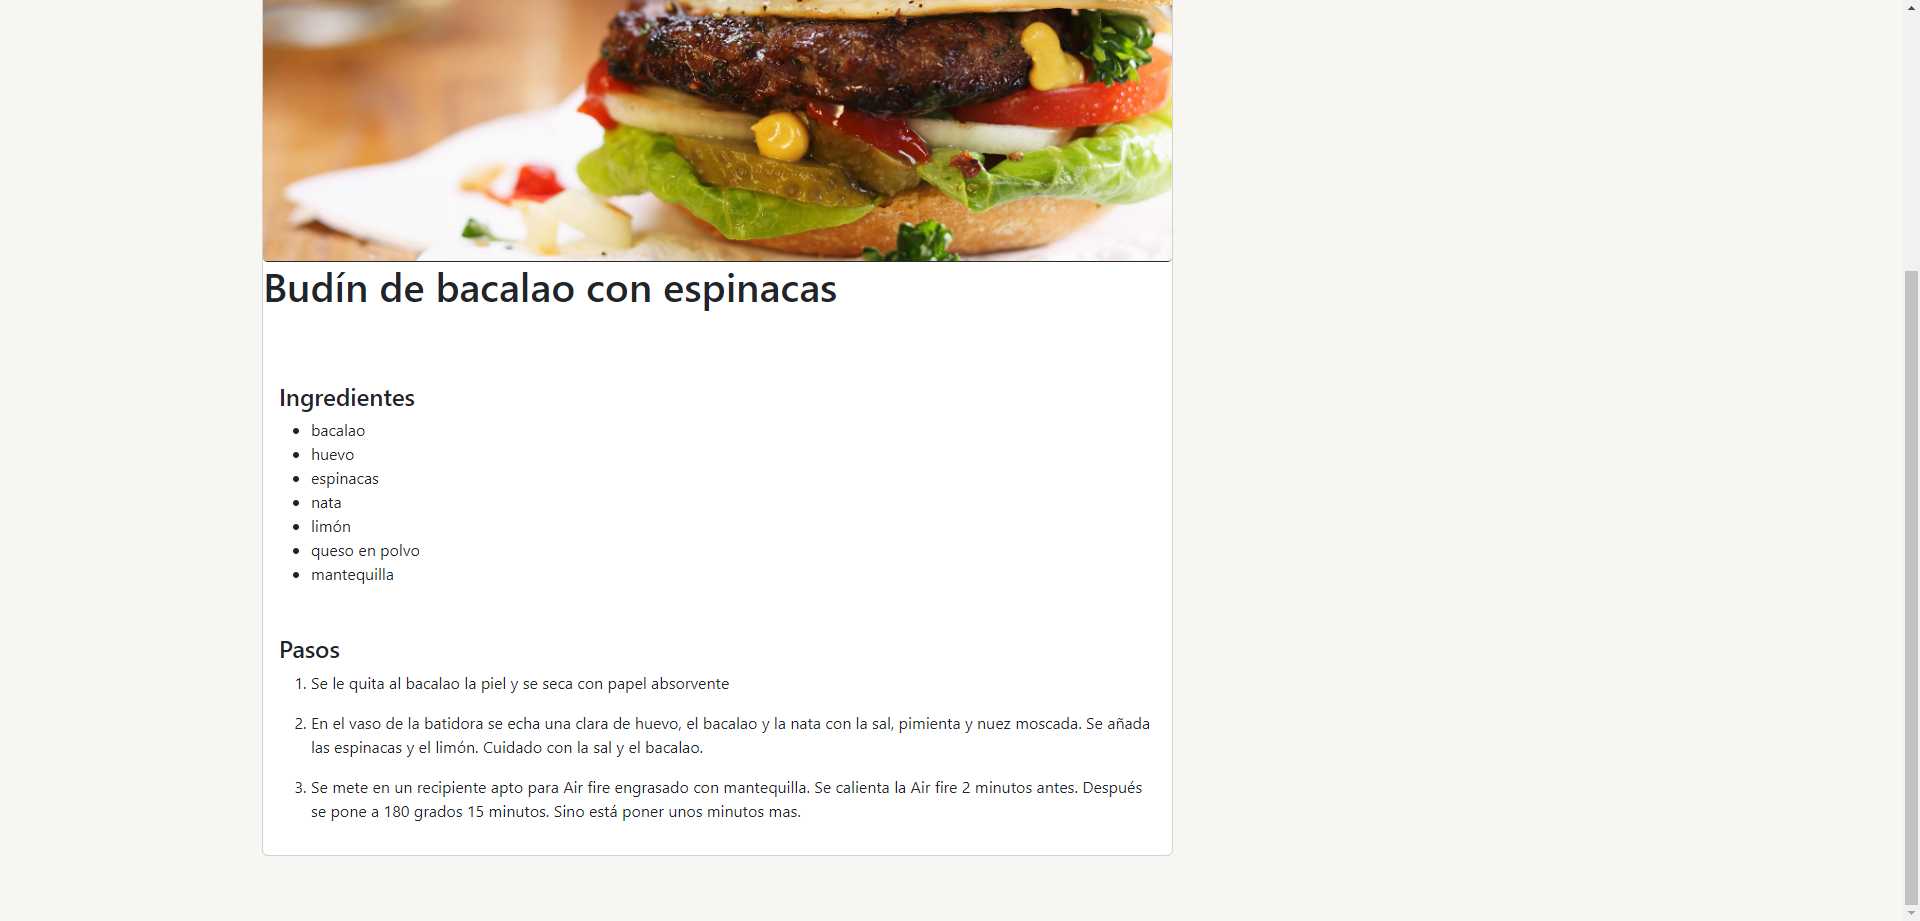
\includegraphics[width=120mm, scale=1]{./doc/imagenes/Recetafinal_Daniel.png}}
    \caption{Pasos finales de Daniel}
    \label{fig:Daniel-pasos2}
\end{figure}

Otro viaje por la aplicación es el de María Encarnación, al que su hijo recomienda usar la aplicación y se la muestra en su tableta, enseñándola a usarla. Observa el buscador inicial, incluyendo algunos ingredientes, pero no quiere buscar recetas por ingredientes, así que los elimina todos con el botón ``Eliminar selección''. Para buscar recetas por nombre su hijo le dijo que tenía que utilizar la barra de arriba, así que busca ``Bizcocho''. 

\begin{figure}[H]
    \fbox{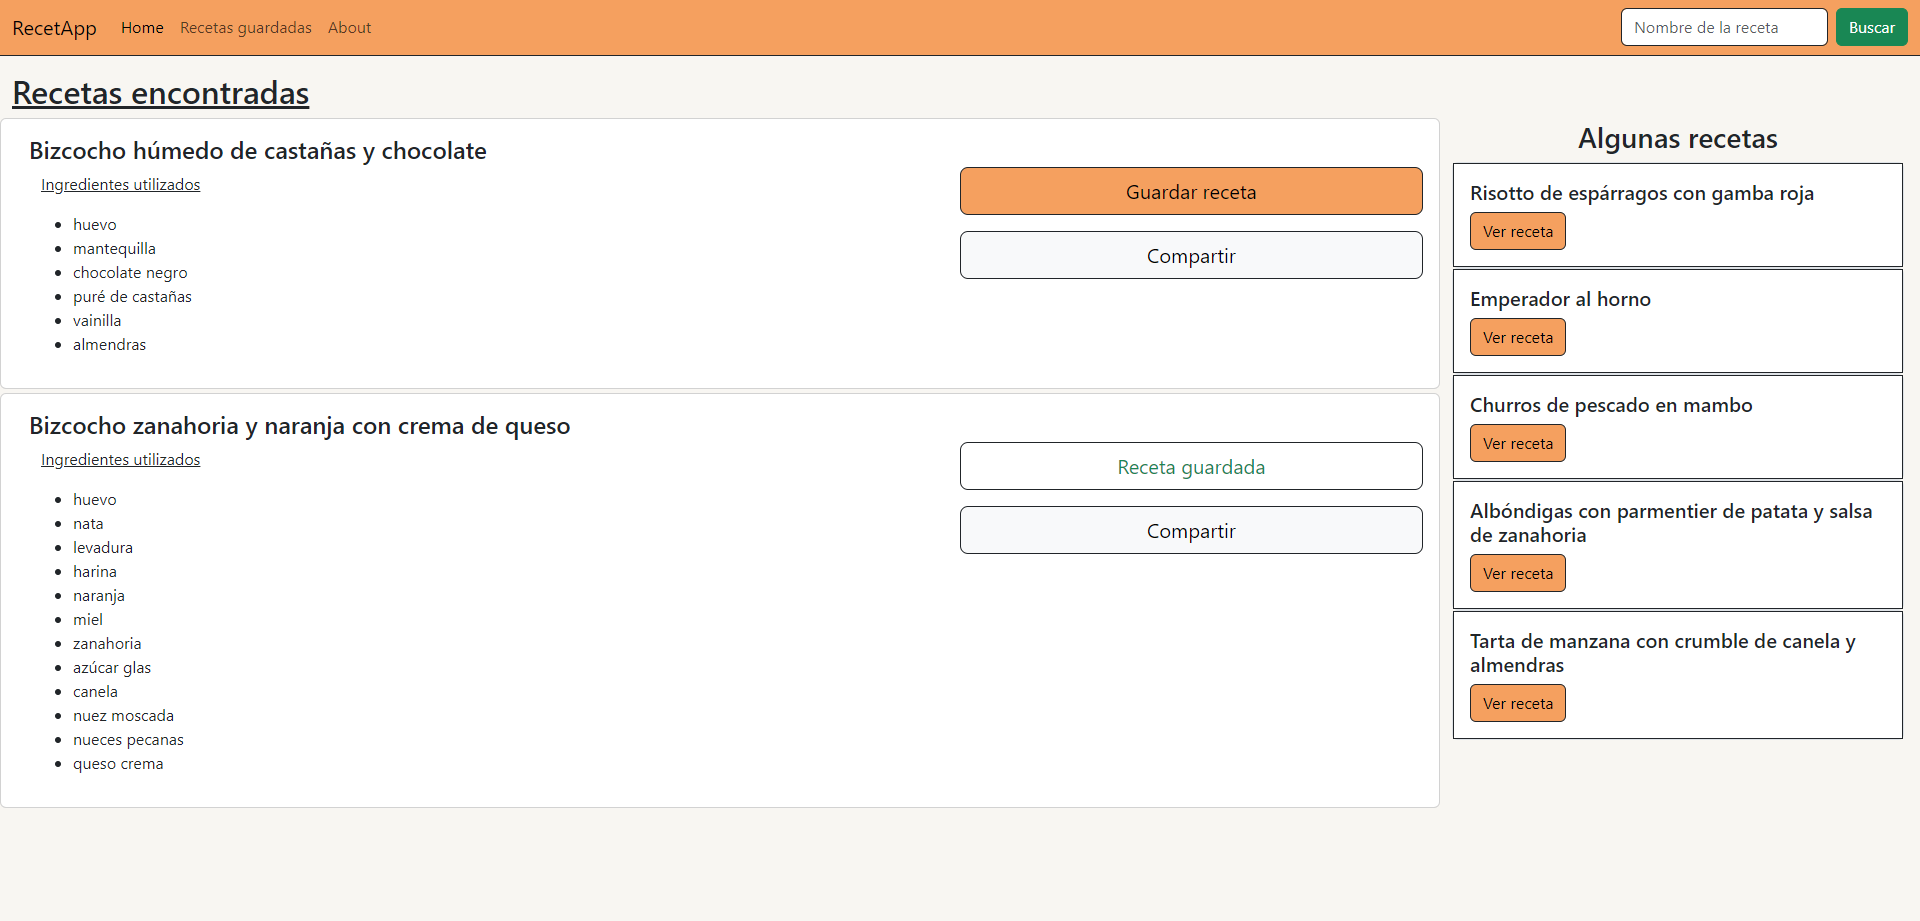
\includegraphics[width=120mm, scale=1]{./doc/imagenes/Resultados_Marien.png}}
    \fbox{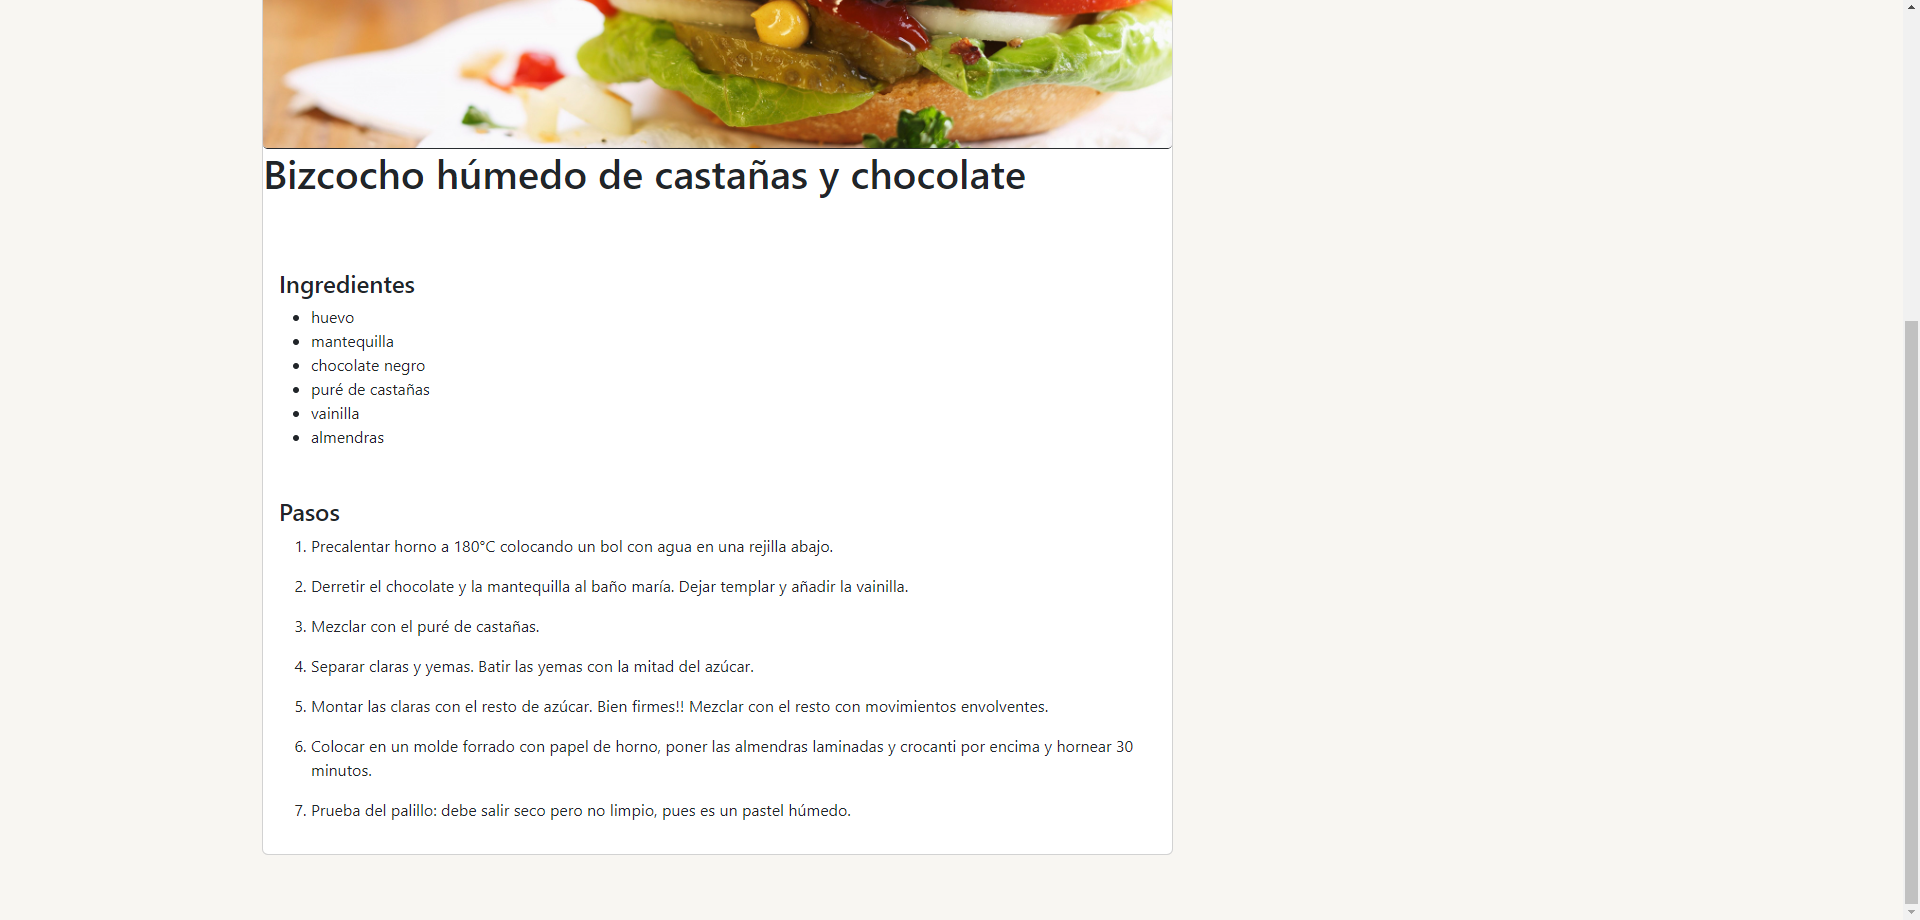
\includegraphics[width=120mm, scale=1]{./doc/imagenes/bizcocho.png}}
    \caption{Resultados a la búsqueda de María Encarnación}
    \label{fig:Daniel-pasos2}
\end{figure}

Decide escoger el bizcocho húmedo de castaña y guardar el de zanahoria para otro día.

Con esta interfaz se recogerán las opiniones de los usuarios tanto para mejorar la funcionalidad como para mejorar esta interfaz final. En conclusión, la \gls{interfaz} funciona correctamente y de la manera esperada para el uso de los usuarios, tanto para estudiantes que necesitan restringir la búsqueda de recetas para incluir solo recetas que puedan hacer con los ingredientes que tienen como para usuarios mayores que no recuerdan las recetas con exactitud.
